\section{Spiel Algorithmus} 

\subsection{Strategie}

\subsection{KI}

Ist nicht direkt teil unseres Konzepts, aber wir müssen der KI gewisse Informationen zur verfügung stellen damit sie überhaupt operieren kann.

Dazu gehören:

Spiel Start Signal
Stapel in der mitte des Spielfelds
Die Handkarten des Spielers
Das Legen einer Karte auf einen Stapel (Erfolgreich oder nicht)
Spiel End Signal
Punkte Abrechnungs Informationen

\subsection{Ablaufdiagramm}

1. dä Server verwaltet diä KartenStapel wo i dä mitti vom spielfeld sind
			2. dä Server hät am afang pro spieler 40 karten wo vorsortiert sind diä muäs är irgendwiä äm jewiligä spieler übergä
			3. sobald diä karte übergä sind übernimmt dä client d kontrolle über diä chartene
			4. dä client baut sin ligretto stapel, + sini 4 offne charte und seit dänn am Server, dass er Ready isch
			5. dä server wartet bis alli Ready sind und macht dänn äs Startsignal
			6. jede client fangt jetzt a regelmässig dä zuästand vo dä Stapel i dä Mitti abzfragä und versuächt sini chartene z spiele.
			7. Wenn er ä möglichkeit gseet versuächt er ä charte am Server z übergä für än gwüssä Stapel. Er wartet bis dä Server meldet ob das klappt hät oder nöd
			8. Sobald das klappt hät macht er wiiter, wänns nöd klappt hät chunt er vom Server sini Charte zrugg über und muäs si wieder detä härä legä wo si gsi isch.
			nachdem ein spieler sin ligretto stapel fertig hät macht er irgend äs Ligretto Stop signal. dä Server leitet das wiiter a alli spieler und returnt no alli charte wo erst nach däm ligretto stop signal acho sind.
			jede spieler zellt jetzt sin ligretto stapel und meldet diä zahl an Server
			dä Server sortiert alli karte, zellt si und verrechnet jetzt diä pünkt.
			
\begin{figure}[hbt]
  \centering
  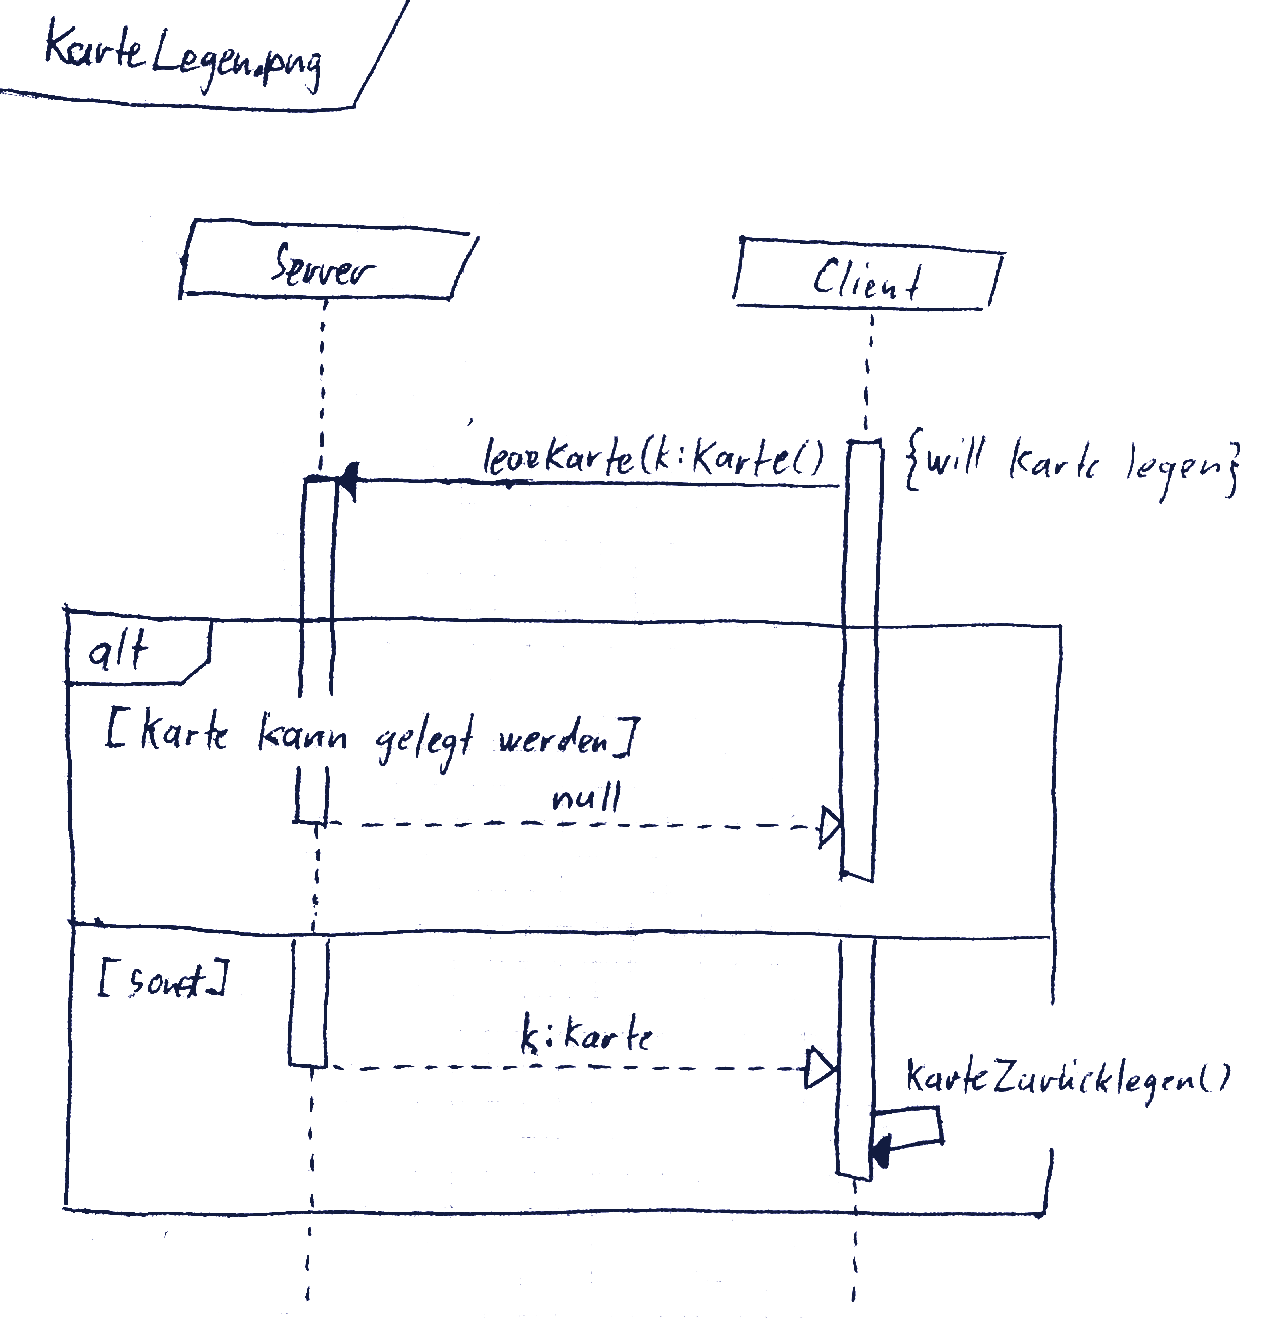
\includegraphics[width=0.80\textwidth,angle=0]{graphics/KarteLegen.png}
  \caption{Sequenzdiagramm zum Legen einer Karte [Papier und Stift FTW] \hfill{} }
 \end{figure}
